%!TEX TS-program = lualatex
%!TEX encoding = UTF-8 Unicode

\documentclass{beamer}

\usepackage{fontspec}
\usepackage{polyglossia}
\setdefaultlanguage{english}
\setotherlanguage{swedish}
\usepackage[english]{selnolig}

\usepackage{csquotes}
\usepackage{microtype}
%\usepackage{beamerthemesplit}

%\usepackage{pdfpages}
%\usepackage[natbib=true,citestyle=numeric]{biblatex}
%\usepackage{rotating}

%\usepackage{tikz}
%\usetikzlibrary{shapes}
%\usetikzlibrary {positioning}
%\definecolor {processblue}{cmyk}{0.96,0,0,0}

\usepackage{graphicx}
\usepackage{minted}

%\usenavigationsymbolstemplate{}
\usetheme{Luebeck}

%\usepackage{beamerthemeIntel}
\setbeamercolor{background canvas}{bg=}	% required for includepdf

%\bibliography{../paper/reflist.bib}

\title[File System Manipulation for Virtual Platforms]{File System Manipulation for Virtual Platforms}
\subtitle{}
\author{Andreas Gnau}
\date{\today}

% BEGIN: speaker notes on the right (comment to hide notes)
% can be comfortably views with dspdfviewer (Linux)
% ==> seems to work on Mac as well, but needs to be compiled
% or Skim (Mac) http://skim-app.sourceforge.net/
\def\shownotesright{}
\ifdefined\shownotesright
\usepackage{pgfpages}
\setbeameroption{show notes}
\setbeameroption{show notes on second screen=right}
\else\ifdefined\shownotesonly
\setbeameroption{show only notes}
\fi
\fi

% END: speaker notes on the right


\usepackage{hyperref}
\hypersetup{pdfusetitle, colorlinks=false, hidelinks}
% pdfpagemode=FullScreen


% uncomment below (and comment above) to print the notes only
%\setbeameroption{show only notes}

\begin{document}

    %!TEX TS-program = xelatex
%!TEX encoding = UTF-8 Unicode

%\frame[plain]{ % When including a large figure or table, you don't want to have the bottom and the top of the slides.
%\frame[shrink]{ % If you want to include lots of text on a slide, use the shrink option.

% Explain why we did this research
\frame[plain]{
\titlepage
\note{
    \begin{itemize}
%        \item probably wondered why I sound so strange when speaking Swedish
%        \item German
%        \item I have been consultant for software after my bachelor's
%        \item after three years, decided to get adventurous and study in Sweden 
        \item My name is Andreas Gnau.
        \item work at Sylog a consultant company and Embedded Linux is what I am mostly dealing with.
        \item and today I will tell you about a project called Linux Kernel Library
        \item and how it can be used to re-use Linux-kernel fs drivers
        \item run in user space
    \end{itemize}
}

}


    \section[Outline]{}
        \frame{\tableofcontents \note{note text}}
    \section{Introduction}
        %!TEX TS-program = xelatex
%!TEX encoding = UTF-8 Unicode

%\frame[plain]{ % When including a large figure or table, you don't want to have the bottom and the top of the slides.
%\frame[shrink]{ % If you want to include lots of text on a slide, use the shrink option.

% Explain why we did this research

\begin{frame}

    \frametitle{Introduction}
    
    Virtual machines are widely used for development.

    Exchanging files while the guest (VM) running is not always feasible or possible, e.g. when...
    \begin{itemize}
        \item bootstrapping a new guest
        \item the guest not providing any networking
        \item the guest is paused during debugging
    \end{itemize}

    \note{
        \begin{itemize}
            \item VM enable a single host hardware to run multiple different guest OS isolated from another.
            \item exchanging files done while VM is running using NW or hypervisor-specific tools
            \item online not always feasible or possible
            \begin{itemize}
                \item bootstrapping a new guest (exchanging executable using a script)
                \item no networking or HV-specific support is available on the target (BIOS development)
                \item debugging: getting debugging symbols. Breakpoint
            \end{itemize}
        \end{itemize}
    }
\end{frame}
        %!TEX TS-program = xelatex
%!TEX encoding = UTF-8 Unicode

%\frame[plain]{ % When including a large figure or table, you don't want to have the bottom and the top of the slides.
%\frame[shrink]{ % If you want to include lots of text on a slide, use the shrink option.

\begin{frame}

\frametitle{Introduction}
    \begin{block}{Goal:}
        \begin{itemize}
        \item provide CLI and native filesystem access on both Windows and Linux
        \item uniform interface, regardless of file system type
        \item provide support for file systems not supported by the host OS
        \item keep extensibility in mind with regards to file systems supported
        \end{itemize}
    \end{block}

    \note{
        \begin{itemize}
            \item provide CLI and native filesystem access on both Windows and Linux
            \item uniform interface, regardless of file system type
            \item not only filesystems supported by host
            \item re-use existing implementations, keep extensibility in mind
        \end{itemize}
    }
\end{frame}
        %!TEX TS-program = xelatex
%!TEX encoding = UTF-8 Unicode

%\frame[plain]{ % When including a large figure or table, you don't want to have the bottom and the top of the slides.
%\frame[shrink]{ % If you want to include lots of text on a slide, use the shrink option.

\frame[t] {
    
    \frametitle{Existing Solutions}
    \begin{columns}[t]
        \begin{column}{.45\textwidth}
            \begin{block}{Linux}
                \begin{itemize}
                    \item loopback-mounting
                    \item filesystem-specific CLI-utilities (e.g. mtools)
                    \item alternative drivers (kernel and FUSE)
                    \item libguestfs
                    \item Linux Kernel Library (LKL)
                \end{itemize}
            \end{block}
        \end{column}
        \begin{column}{.55\textwidth}
            \begin{block}{Windows}
                \begin{itemize}
                    \item mounting VHD-files
                    
                    \item filesystem-specific CLI-utilities (e.g ltools)
                    \item alternative drivers (kernel and FUSE)
                \end{itemize}
            \end{block}
        \end{column}
    \end{columns}
    \note{
        \begin{itemize}
            \item loopback/VHD mounting, => standard native way, included with OS, limited to OS FS support
            \item filesystem-specific CLI-utilities (mtools, ltools) => non-uniform interface, re-implementation, less-proven code
            \item alternative drivers may lack the stability and feature-set of mature implementations
            \item Only libguestfs offers wide-FS support under a uniform interface. Goal: re-use OS-level code!
            \item LKL (allows using the Linux Kernel as a library)
        \end{itemize}
    }
}
    \section{Background}
        %!TEX TS-program = lualatex
%!TEX encoding = UTF-8 Unicode

%\frame[plain]{ % When including a large figure or table, you don't want to have the bottom and the top of the slides.
%\frame[shrink]{ % If you want to include lots of text on a slide, use the shrink option.

\begin{frame}
    \frametitle{FUSE (File System in User Space)}
    \begin{center}
        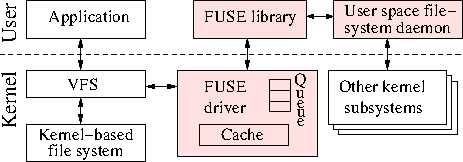
\includegraphics[width=.7\textwidth]{frames/img/fuse_arch}
    \end{center}
    
    \begin{itemize}
        \item simplifies writing file system drivers by avoiding kernel-level code
        \item mounting / unmounting can be done as an unprivileged user
        \item file ownership can be adjusted to enable unprivileged access to the filesystem
    \end{itemize}
    
    \note{
    \begin{itemize}
        \item kernel driver exposes a queue of requests to user space...
        \item ... which is consumed by a user space daemon handling those requests
        \item Of course there is some overhead due to context switches and copying
        \item simplifies writing file system drivers by avoiding kernel-level code
        \item mounting / unmounting can be done as a unprivileged user
        \item file ownership can be adjusted to enable unprivileged access to the filesystem
    \end{itemize}
    }
\end{frame}
        %!TEX TS-program = lualatex
%!TEX encoding = UTF-8 Unicode

%\frame[plain]{ % When including a large figure or table, you don't want to have the bottom and the top of the slides.
%\frame[shrink]{ % If you want to include lots of text on a slide, use the shrink option.

\begin{frame}
    \frametitle{libguestfs}
    \begin{itemize}
        \item library and suite of utilities for offline FS access
        \item uses a dedicated VM for filesystem access
        \item mature ecosystem, many useful CLI utilities
        \item FUSE filesystem available as well, but very slow
    \end{itemize}

\begin{center}
    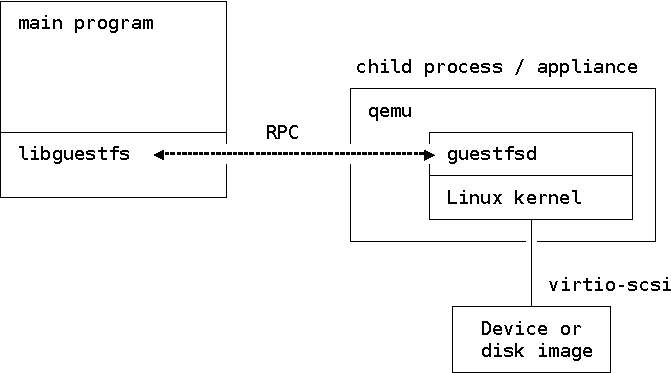
\includegraphics[width=.65\textwidth]{frames/img/libguestfs_arch}
\end{center}
    
    \note{
        \begin{itemize}
            \item \textbf{Q} library and suite of utilities for offline FS access
            \item Approach: runs a small virtual machine with  Linux that does the FS-access
            \item process on the host talks to process in the VM
            \item quite some overhead, but the goal is to isolate the operations from the host
            \item fast CLI utils, slow FUSE => additional overhead, because data is transferred in smaller chunks
        \end{itemize}
    }
\end{frame}
        %!TEX TS-program = xelatex
%!TEX encoding = UTF-8 Unicode

%\frame[plain]{ % When including a large figure or table, you don't want to have the bottom and the top of the slides.
%\frame[shrink]{ % If you want to include lots of text on a slide, use the shrink option.

\begin{frame}
    \frametitle{Linux Kernel Library (LKL)}
        \begin{columns}[c]
            \begin{column}{.45\textwidth}
                \begin{itemize}
                    \item arch-port of the Linux kernel
                    \item only basic primitives are implemented on the host side (threading, TLS, semaphores, timers...)
                    \item CLI-utilities and experimental FUSE exist
                \end{itemize}
            \end{column}
            \begin{column}{.55\textwidth}
%\includegraphics[width=.9\textwidth]{frames/img/lkl_overview}
            \end{column}
        \end{columns}


    \note{
        \begin{itemize}
            \item arch-port similiar to UML to enable use as a library
            \item interface is the syscalls, e.g. lkl\_sys\_getpid()
            \item basic primitives are implemented for each host, POSIX, Win32, Windows Kernel, Haiku OS
            \item interesting use cases EFI filesystem driver, running LKL inside a SGX enclave etc.
        \end{itemize}
    }
\end{frame}

    \section{Contribution}
        %!TEX TS-program = lualatex
%!TEX encoding = UTF-8 Unicode

%\frame[plain]{ % When including a large figure or table, you don't want to have the bottom and the top of the slides.
%\frame[shrink]{ % If you want to include lots of text on a slide, use the shrink option.

\begin{frame}

\frametitle{Implementation}
\begin{itemize}
    \item ported LKL CLI-utilities for FS manipulation to Windows
    \item ported lklfuse to Windows and brought it to (near-)production quality on Linux
    \item[$\Rightarrow$] We can now mount any filesystem supported by the Linux Kernel under Windows
    \item created an experimental backend for libguestfs based on LKL
    \item tried to port libguestfs to Windows (time was too short to accomplish that)
    %\item \textbf{TODO: ??? Add architecture diagram of lklfuse and libguestfs-lkl-fuse here }
\end{itemize}

\note{
\begin{tiny}

    \begin{itemize}
        \item So, what did \textbf{I} do (besides evaluating)?
        \item ported LKL-utils
        \item lklfuse for Windows and Linux
        \begin{tiny}

        \begin{itemize}
            \item \tiny{]can now handle load (LKL is limited to 32/64 syscall threads and those threads were not freed...). Took two attempts to get right. Now the limit has been raised to 1024 / 4096 threads upstream}
            \item \tiny{large file support (Did you know how Kernel >= 2.6 handle LFS?). I needed to find out by stepping from the VFS-layer to EXT4 to MM...}
            \item resource leaks on Windows
            \item \tiny{bugfixes in Dokan-FUSE (e.g. rmdir a directory with files in it => returned success even though it was not deleted)}
            \item \tiny{using command-line-arguments to enable caching, bigger writes}
        \end{itemize}
        \end{tiny}
        \item libguestfs LKL backend: quick and dirty implementation, too slow for practical use, needs further investigation


        \begin{itemize}
            \item \tiny{how to port the code from using open() to lkl\_sys\_open()? Looked into objcopy, coccinelle, manual editing, ifdefs. Ended up doing many \#defines}
            \item \tiny{Even the original qemu-KVM is very slow, and so is the LKL-port.}
            \item \tiny{A maintainable solution needs to be found to implement this code-wise}
        \end{itemize}

        \item tried to port libguestfs to Windows (time was too short to accomplish that)
    \end{itemize}
    
\end{tiny}
}


\end{frame}

    \section{Evaluation}
        %!TEX TS-program = lualatex
%!TEX encoding = UTF-8 Unicode

%\frame[plain]{ % When including a large figure or table, you don't want to have the bottom and the top of the slides.
%\frame[shrink]{ % If you want to include lots of text on a slide, use the shrink option.

\begin{frame}

\frametitle{Evaluation: The How}
\begin{itemize}
    \item challenge: find balance between evaluating for our use case and general applicability
    \item focus on synthetic benchmarks for a start, fits the use case of exchanging one or two files
    \item using extensive suite of existing benchmarks (Filebench) not possible due to missing Windows support
    \item to be expected that performance will be worse under real-world workloads
\end{itemize}

\note{
    \begin{tiny}
    \begin{itemize}
        \item challenge: find balance between evaluating for our use case (mounting images) and general applicability (mounting disks, production use)
        \item There exists only one good paper evaluating FUSE performance
        \item would have been really nice to reproduce the results of that paper in addition and in comparison to LKL-based file systems
        \item focus on synthetic benchmarks for a start, fits the use case of exchanging one or two files
        \item to be expected that performance will be worse under real-world workloads
        \item What:
        \begin{tiny}
        \begin{itemize}
            \item RAM reduced to 4GB, 16 GB file size, empty Ext4 FS of  33 GB
            \item Linux: loopback-mounting, LKL-FUSE, libguestfs-KVM, libguestfs-LKL
            \item Windows: LKL-FUSE (Dokany), VHD with NTFS
        \end{itemize}.
        \end{tiny}
    \end{itemize}
\end{tiny}
}


\end{frame}

        
%!TEX TS-program = lualatex
%!TEX encoding = UTF-8 Unicode

%\frame[plain]{ % When including a large figure or table, you don't want to have the bottom and the top of the slides.
%\frame[shrink]{ % If you want to include lots of text on a slide, use the shrink option.


\begin{frame}[plain]
    \frametitle{Throughput Relative to Linux Loopback Mounting}
    \vspace*{-1pt}
    \makebox[\linewidth]{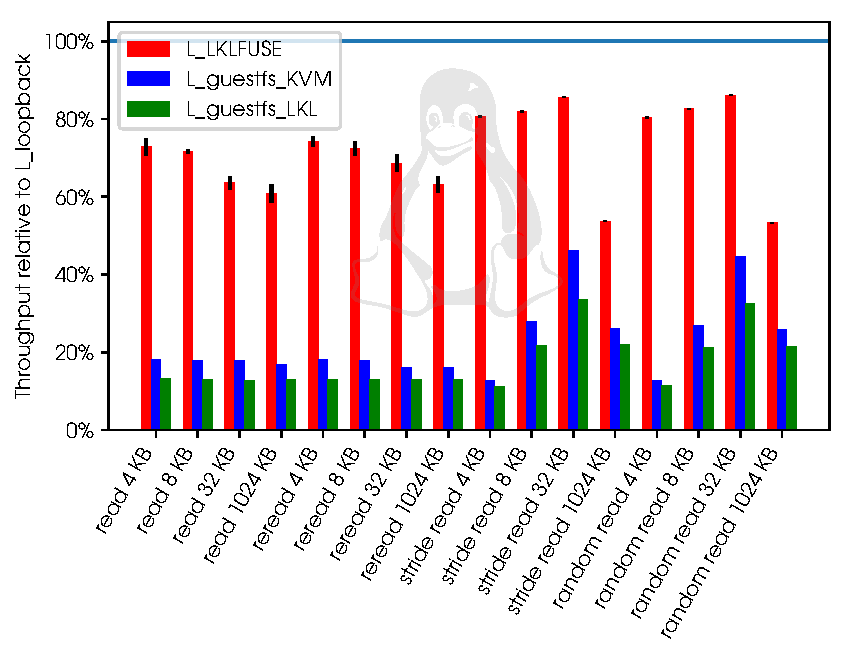
\includegraphics[page=1,width=0.87\paperwidth]{frames/img/relative_performance_filter_read_baseline_L_loopback_variants_L_LKLFUSE_L_guestfs_KVM_L_guestfs_LKL}}
    \note{
        \begin{itemize}
            \item X-axis, workloads, read, reread. stride read, random read
            \item Y-access relative to baseline loopback-mounting
            \item three colors, red LKLFUSE, blue guestfs KVM, green guestfs LKL
            \item LKLFUSE delivers okay read performance, i.e. 72\%
            \item very consistent irregardless of blocksize. readahead
            \item loopback has readahead as well. possible that amplification occurrs over several layers
            \item less pronounced effect for stride and random read
            \item libguestfs is too slow. architecture not made for FUSE but CLI.
            \item mostly caused by the communication protocol overhead.
            \item guestfs-LKL worse than KVM around 80\%. Profiling needed
            \item I expect it to be possible to optimize the prototypic LKL-backend so that it outperforms the LKL-backend

        \end{itemize}
    }
\end{frame}

\begin{frame}[plain]
\frametitle{Throughput Relative to Linux Loopback Mounting}
\vspace*{-1pt}
\makebox[\linewidth]{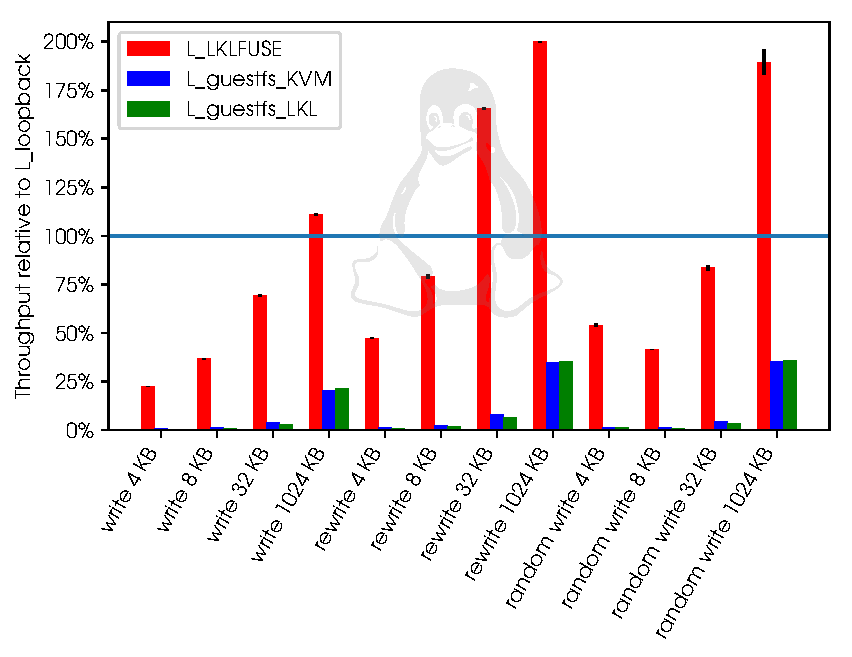
\includegraphics[page=1,width=0.87\paperwidth]{frames/img/relative_performance_filter_write_baseline_L_loopback_variants_L_LKLFUSE_L_guestfs_KVM_L_guestfs_LKL}}
\note{
    \begin{itemize}
        \item LKLFUSE: seq write delivers okay performance, i.e. above 50\%
        \item big difference between blocksizes. Overhead of each write reaching the FS one by one
        \item much better than baseline: how is that possible. No fsync!
        \item writing to pages that have not been written back (rewrite, random write), writeback caching
        \item FUSE does not have it, but the lower layers (LKL and read of image)
        \item many moving parts, two kernels, several caches, readahead...
        \item libguestfs-lkl is too slow
        \item mostly caused by the communication protocol overhead.
        \item libguestfs-kvm is only slightly faster
        \item I expect it to be possible to optimize the prototypic LKL-backend so that it outperforms the LKL-backend
        
    \end{itemize}
}
\end{frame}

\begin{frame}[plain]
    \frametitle{Throughput Relative to Windows VHD Mounting}
    \vspace*{-1pt}
    \makebox[\linewidth]{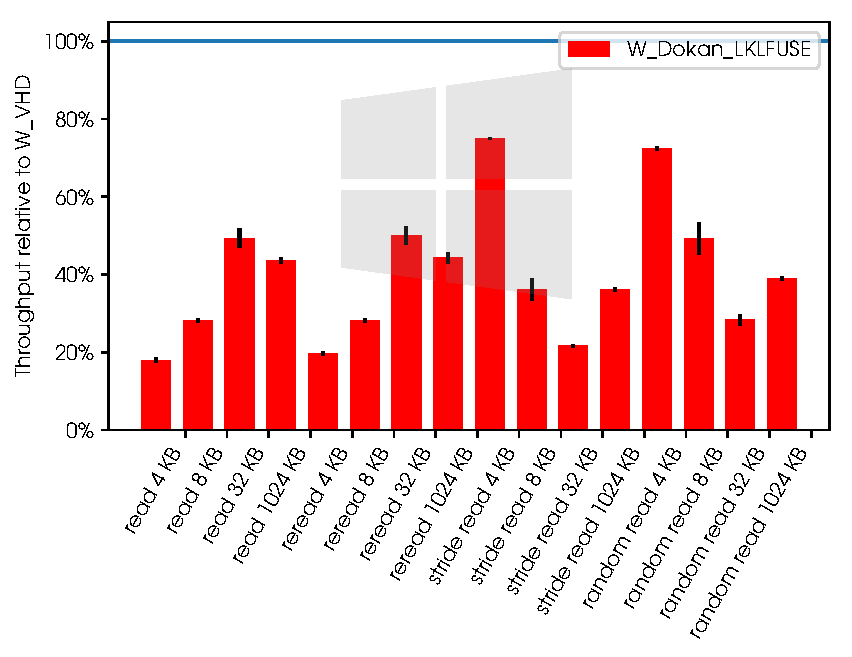
\includegraphics[page=1,width=0.87\paperwidth]{frames/img/relative_performance_filter_read_baseline_W_VHD_variants_W_Dokan_LKLFUSE}}
    \note{
        \begin{itemize}
            \item LKLFUSE-Dokan does worse in relative (and absolute) under Windows than under Linux.
            \item 40\% on average read performance. in opposite to Linux, higher blocksizes help, no readahead
            \item Dokan has several problems (no caching, fixed number of worker threads)
            \item interesting differences between blocksizes, not bigger is better. does not go through caching layer
            \item LKL maybe also has some room improvement, Windows API expert
        \end{itemize}
    }
\end{frame}

\begin{frame}[plain]
\frametitle{Throughput Relative to Windows VHD Mounting}
\vspace*{-1pt}
\makebox[\linewidth]{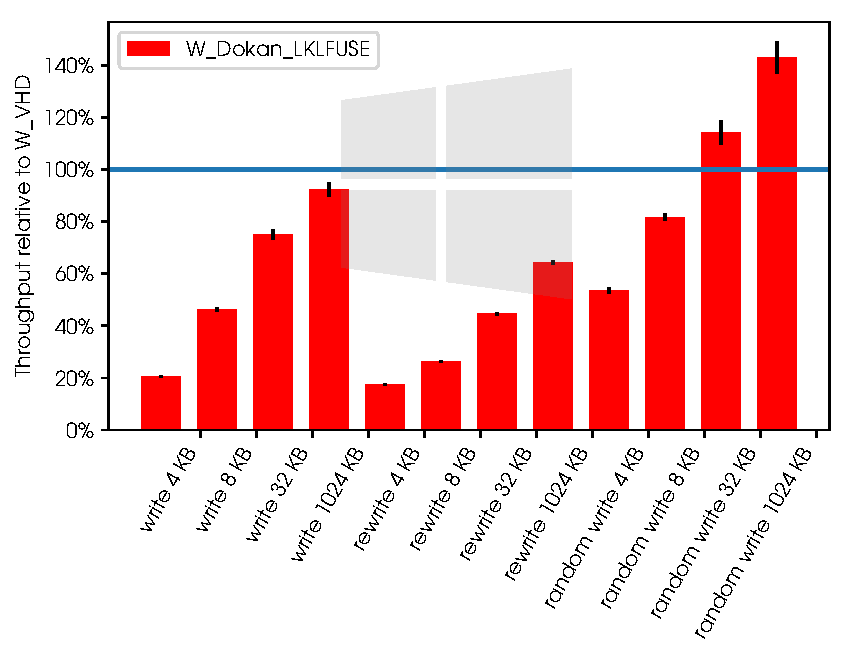
\includegraphics[page=1,width=0.87\paperwidth]{frames/img/relative_performance_filter_write_baseline_W_VHD_variants_W_Dokan_LKLFUSE}}
\note{
    \begin{itemize}
        \item write 65\%, in-line with read-workloads. Differences for different blocksizes
        \item also outperforming for random reads
    \end{itemize}
}
\end{frame}

    \section{Conclusion}
        %!TEX TS-program = lualatex
%!TEX encoding = UTF-8 Unicode

%\frame[plain]{ % When including a large figure or table, you don't want to have the bottom and the top of the slides.
%\frame[shrink]{ % If you want to include lots of text on a slide, use the shrink option.

\begin{frame}

\frametitle{Conclusion}
\begin{itemize}
    \item LKLFUSE delivers acceptable performance for the use case of exchanging files from disk images on Linux
    \item LKLFUSE on Windows is held back by the lack of good userspace FS library
    \item more evaluation and optimizations needed for more general-purpose use
    \item dedicated command-line utilities deliver higher performance but depending on the use case a worse user experience
    \item libguestfs is a very useful toolset in its current form, but is best used from command-line
    \item time was too short to analyse the results in detail
\end{itemize}

\note{
    \begin{itemize}
    \item LKL delivers acceptable performance for the use case of exchanging files from disk images
    \item LKLFUSE on Windows is held back by the lack of good userspace FS library
    \item More evaluations and optimizations are needed for more general-purpose use
    \item Use dedicated tools for performance, FUSE for usability
    \item libguestfs is a very useful toolset in its current form wrt. to its feature-set
    \item libguestfs architecture not suited for FUSE use case or LKL


    \end{itemize}
}


\end{frame}

        %!TEX TS-program = xelatex
%!TEX encoding = UTF-8 Unicode

%\frame[plain]{ % When including a large figure or table, you don't want to have the bottom and the top of the slides.
%\frame[shrink]{ % If you want to include lots of text on a slide, use the shrink option.

\begin{frame}

\frametitle{Recommendations and Ideas}
\begin{itemize}
    \item simplify the documentation on loopback mounting
    \item port SimicsFS to Windows using Dokan
    \item enable on-the-fly access to CRAFF-images from the host using CRAFF-FS (FUSE) or some other technique like NBDkit
    \item link CRAFF-FS to Dokan-FUSE and expose a VHD for mounting on Windows
    \item make the libguestfs-appliance run on Simics
    \item enable downloading of debug-symbols from the target using checkpointing and/or some of the technologies presented
\end{itemize}

\note{
\begin{itemize}
    \item simplify the documentation on loopback mounting (currently involves running parted and calculating offsets)
    \item port SimicsFS to Windows using Dokan or another FUSE library
    \item enable on-the-fly access to CRAFF-images from the host using CRAFF-FS (FUSE) or some other technique like NBDkit
    \item link CRAFF-FS to Dokan-FUSE and expose a VHD for mounting on Windows
    \item make the libguestfs-appliance run on Simics
    \item enable downloading of debug-symbols from the target using checkpointing and/or some of the technologies presented
\end{itemize}
}


\end{frame}

%    \section*{Backup Slides}
        %!TEX TS-program = xelatex
%!TEX encoding = UTF-8 Unicode

%\frame[plain]{ % When including a large figure or table, you don't want to have the bottom and the top of the slides.
%\frame[shrink]{ % If you want to include lots of text on a slide, use the shrink option.

\begin{frame}
    
    \frametitle{Thanks!}
        \begin{center}
            \huge{Questions?}
        \end{center}
    \note{
        \begin{itemize}
            \item like it here
            \item learned a lot
            \item scope was too wide, lklfuse + utils would have been enough
            \item could have asked for help more often
            \item thank everyone who made me feel welcome, gave advice, talked Swedish with me even if it was a bit of a hassle
            \item learned to work in Sweden
        \end{itemize}
         }
    
    
    
\end{frame}


\begin{frame}

\frametitle{Backup Slides}
    
\note{note text}



\end{frame}



        %!TEX TS-program = xelatex
%!TEX encoding = UTF-8 Unicode

%\frame[plain]{ % When including a large figure or table, you don't want to have the bottom and the top of the slides.
%\frame[shrink]{ % If you want to include lots of text on a slide, use the shrink option.

% Explain why we did this research

\begin{frame}[fragile]
    \begin{listing}[H]
        \begin{minted}{console}
# losetup --find --show --partscan debian8.img
/dev/loop0

# file -s /dev/loop0*
/dev/loop0:   DOS/MBR boot sector
/dev/loop0p1: Linux rev 1.0 ext4 filesystem data, UUID=b90f0480-a8b5-4369-a2c5-31d005477b10 (extents) (large files) (huge files)
/dev/loop0p2: DOS/MBR boot sector; partition 1 : ID=0x83, start-CHS (0x17a,28,35), end-CHS (0x233,120,5), startsector 2, 2977792 sectors; partition 2 : ID=0x5, start-CHS (0x233,120,6), end-CHS (0x273,184,5), startsector 2977794, 1032192 sectors, extended partition table
/dev/loop0p5: Linux rev 1.0 ext4 filesystem data, UUID=48308279-ef74-4d5e-8c14-547d7178afa3 (extents) (large files) (huge files)
/dev/loop0p6: Linux/i386 swap file (new style), version 1 (4K pages), size 128767 pages, no label, UUID=963e44b9-9534-4a0f-8d63-5006653bf40a
/dev/loop0p7: Linux rev 1.0 ext4 filesystem data, UUID=4c5efdb6-6647-437d-99db-86f33a8ca417 (extents) (huge files)
/dev/loop0p8: Linux rev 1.0 ext4 filesystem data, UUID=d7f0d2c9-1a40-4c06-8c68-374c3ad45ee6 (needs journal recovery) (extents) (large files) (huge files)

# mount /dev/loop0p5 /mnt/mountpoint
        \end{minted}
    
        \caption{Recent versions of util-linux allow creating loop-devices for individual partitions}

        \label{lst:mount_loop}
    \end{listing}
    
\note{
    \begin{itemize}
        \item Mounting images without partition table (filesystem images)% \mintinline{console}{# mount -o loop img /mnt} works fine}
        \item If the loop-/sys/module/loop/parameters/max\_part
        \item Older versions of util-linux do not support the --partscan-parameter which will instruct the kernel to read the partition table. The partprobe-command from libparted can be a replacement in this case. On kernels older than 3.2, the loop module has to be loaded with a non-zero max\_part parameter.
        https://git.kernel.org/cgit/utils/util-linux/util-linux.git/commit/?id=59d749c33136b85fc4a51a0af6c48cc97e3d1b31
    \end{itemize}
}



\end{frame}



    
%	\input{frames/references.tex}
\end{document}